\chapter{Probabilistic Generative Models}

It is worth highlighting that there are many overlapping definitions and conflicting terminology in the field of generative models~\cite{DiscriminativeVsGenerative, MachineLearningDiscriminative}, so we will attempt to directly define the terms used in this thesis.
We assume the existence of some unknown probability density function $p_\X(\x): \mathcal{X} \rightarrow \mathbb{R}$ over some random variable $\X \in \mathcal{X}$ which is used to populate a dataset $\mathcal{D} = \{\x_i\}_{i=1}^N$.
A probabilistic generative model (PGM) is a parametrized model fit using $\mathcal{D}$ that allows for the efficient generation of new samples following the same distribution.
There exist many types of PGMs, and some like Generative Adversarial Networks (GANs)~\cite{GenerativeAdversarialNetworks} only allow for the generation of samples, while others like Normalising Flows (NFs)~\cite{VariationalInferenceNormalizing} provide an explicit approximation of the density $p_{\theta}(\x) \approx p_\X(\x)$.

Quite often we are also interested in approximating a conditional distribution $p_{X}(\x|\con)$ where $\con$ is some context variable.
This is useful for many tasks in machine learning, such as text-to-image generation~\cite{Dalle}.
We can also describe supervised learning as conditional generation and the building PGMs where, in contrast to the notation in \Cref{ch:supervised}, $\x$ is now the target variable and $\con$ is the input data.

In this section we cover the theory behind PGMs used in later in this thesis, namely NFs and denoisers.
Here, denoisers is an umbrella term we use to describe the collection of diffusion models~\cite{DDPM, DDIM}, score-based models~\cite{ScoreBasedGenerativeModeling, ElucidatingDesignSpace} flow matching models~\cite{FlowStraightFast, FlowMatchingGenerative} and consistency models~\cite{ConsistencyModels, CM2} all of which share similar training objectives.
These models are all nominally used to generate continuous data, which matches much of the data we are interested in generating in the context of HEP.
Generative models on discrete data, such as the autoregressive models used in text generation~\cite{GPT2} are not included.
An overview of the models is given in \Cref{fig:generative_models}.

\begin{figure}[ht]
    \centering
    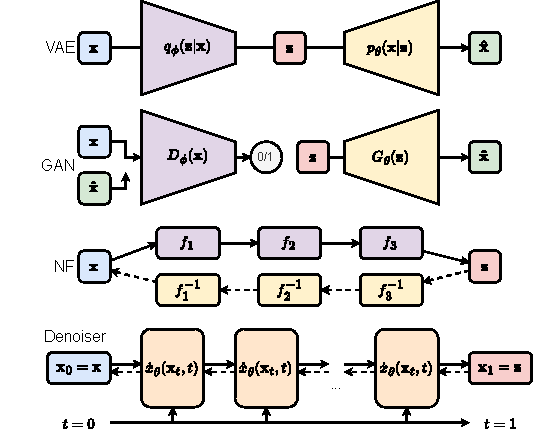
\includegraphics[width=0.8\textwidth]{Figures/transformers/pgms.pdf}
    \caption{An overview of the generative models covered in this thesis.}
    \label{fig:generative_models}
\end{figure}


\section{Older PGMs}

Over the course of this thesis the field of generative models has seen rapid development.
At the start of this thesis, two models dominated the field: Variational Autoencoders~\cite{AutoEncodingVariationalBayes} (VAEs) and GANs~\cite{GenerativeAdversarialNetworks}.
While these older models, especially GANs, produced very impressive results in select domains, the generation quality and fine control of the samples that we see today was not possible.
The current landscape of text-to-image~\cite{Imagen, Dalle, SD3}, and even text-to-video~\cite{ImagenVideo} generation would have been inconceivable just a few years ago.
While it is remarkable how quickly focus of these models has moved on, specifically to denoisers, it is still important to highlight them here, both for historical context and to understand the strengths of the models that have replaced them.

\subsection{Variational Autoencoders}

VAEs were introduced in 2013~\cite{AutoEncodingVariationalBayes} and quickly became a popular model for generative tasks, unsupervised learning and variational inference.
A VAE is an example of a latent variable model.
Here one introduces a latent random variable $\Z \in \mathcal{Z}$ which one marginalizes over to obtain the distribution of the data,
\begin{equation}
    p_\X(\x) = \int p_{\X,\Z}(\x, \z)\diff\z = \int p_\X(\x|\z)p_\Z(\z)\diff\z.
\end{equation}
The latent space usually covers all real values, $\mathcal{Z} = \mathbb{R}^d$, and the prior $p_\Z(\z)$ is taken to be a simple distribution, such as a diagonal Gaussian $\normal$.
Practically we would like to not enforce what information is stored in the latent variable.
The standard choice for modelling the likelihood is to use a parametrised Gaussian with constant variance,
\begin{equation}
    p_\X(\x|\z) \approx p_{\theta}(\x|\z) = \mathcal{N}(\x; G_{\theta}(\z), \sigma^2 I),
\end{equation}
where $G_{\theta}$ is a neural network called the decoder.

VAEs introduce an additional parametrized distribution to approximate the posterior which is also taken to be Gaussian with a diagonal covariance matrix,
\begin{equation}
    p_\Z(\z|\x) \approx q_\phi(\z|\x) = \mathcal{N}(\z; \boldsymbol{\mu}_\phi(\x), \boldsymbol{\Sigma}_\phi(\x)).
\end{equation}
Here the estimation of the mean and variance of the approximate posterior is done by a neural network called the encoder and gradients are backpropagated through the stochastic latent variable using the reparameterisation trick~\cite{AutoEncodingVariationalBayes}.

One can not train this model by simply maximizing the likelihood of the data, as the likelihood is intractable.
However, this form sets up a mapping between the data space to the latent space and back again and one can train the model by maximizing the evidence lower bound (ELBO).
Practically this involves minimizing two terms, the reconstruction loss and the KL-divergence between the approximate posterior and the prior,
\begin{equation}
        \mathcal{L}(\theta, \phi) = \mathbb{E}_{\z \sim q_{\phi}(\z|\x)}[||\x - G_{\theta}(\z)||^2] - \beta D_{KL}(q_{\phi}(\z|\x) || p_\Z(\z)),
\end{equation}
where $\beta$ is a hyperparameter that balances the two terms~\cite{BetaVAE}.

Typically the dimensionality of the latent space is much lower than the data space, so the information bottleneck means the model is forced to learn a compressed representation.
VAEs are simple to train but have a number of limitations.
The bottleneck means that the samples are often of low quality and lacking in high frequency detail.
The model is also sensitive to the tuning of $\beta$, often leading to a collapse into one of two regimes.
Either the prior loss dominates, all samples are encoded to the unit Gaussian and all information is lost.
Alternatively the reconstruction loss dominates, the posterior is non-Gaussian and extra steps are required to sample from it, such as fitting a kernel density estimator to the empirical distribution of the latent variables~\cite{KDEVAE}.

Conditional information can be injected into the VAE simply by combining the context variable with both the inputs to the encoder and decoder.
The compression of the latent means that it only stores orthogonal information to the context variable, which is useful for disentanglement~\cite{cVAE}.

VAEs were never particularly good at generating high quality samples, but they attempts were still made in HEP to use them for fast simulation of detector responses~\cite{VariationalAutoencodersJet, GraphVariationalAutoencoder, ParticlebasedFastJet}.
One other notable usecase for anomaly detection~\cite{VariationalAutoencodersAnomalous, DeepSetVAE, MassiveIssueAnomaly}.
Both of these applications produced mixed results and the field at large has moved on to more powerful models.


\subsection{Generative Adversarial Networks}

Up until recently, GANs were the state-of-the-art in generative models for producing high quality samples.
This was most notably demonstrated in the generation of high resolution images~\cite{StyleGAN2,StyleGAN3}.
GANs are based on a two-player min-max game between a generator $G_\theta(\z)$ and a discriminator $D_\phi(\x)$, each neural networks with parameters $\theta$ and $\phi$ respectively.
These networks contest with each other in a zero-sum game where the one network's loss is the other's gain.

The generator takes a random latent sample $\z \sim p_\Z(\z)$ and returns a synthetic sample $\hat{\x} = G_\theta(\z) \in \mathcal{X}$.
The discriminator takes samples from both the training set and the synthetic samples and returns a probability that the sample is from the training set, $D_\phi(\x) \in [0, 1]$.
The objective of the generator is to fool the discriminator into thinking the generated samples are real.
Given powerful enough networks, the unique Nash equilibrium of this game is a generator that produces the true data distribution and a uniform discriminator output for all real samples.

There are many variations for defining the specifics of this game and the loss functions, but arguably the most widely used is the original non-saturating loss~\cite{GenerativeAdversarialNetworks}.
This loss requires two passes through each network, one to update the discriminator and one to update the generator.
\begin{align}
    \mathcal{L}_{\text{D}}(\phi) &= -\mathbb{E}_{\x \sim \mathcal{D}}[\log D_{\phi}(\x)] - \mathbb{E}_{\z \sim p_\Z(\z)}\log(1 - D_{\phi}(G_{\theta}(\z))], \\
    \mathcal{L}_{\text{G}}(\theta) &= -\mathbb{E}_{\z \sim p_\Z(\z)}[\log D_{\phi}(G_{\theta}(\z))].
\end{align}
Other variants exist which use different loss derivations, such as the Wasserstein GAN~\cite{WGAN1} and the Geometric GAN~\cite{GeometricGAN}.
There is plenty of literature on which variants are best suited for different tasks and which actually converge to the desired Nash equilibrium~\cite{WhichTrainingMethods}.

The main difficulty of GANs is that they are difficult to train.
Often there is mode collapse, where the generator exploits some weakness in the discriminator and reproduces the same samples over and over.
Many tricks are required to stabalize training~\cite{WhichTrainingMethods}, such as minibatch discrimination~\cite{ProGAN} and gradient penalties~\cite{WGAN}.
Another drawback to GANs is that it is difficult to product a conditional generator $G_\theta(\x|\con)$.
Simply concatenating the context variable to both the generator and discriminator inputs leads to mixed results and the generator is prone to ignoring the context variable~\cite{cGAN}.

In HEP, GANs have mainly been trialed as a method for fast simulation~\cite{MPGAN, GAPT, CaloGAN, EPICGAN}.
However, the main issue is that GANs tend to not cover the full data distribution, and that most of the generation we are looking for in fast simulation is conditional;
detector response depends on the properties of the incoming particle, making GANs not optimal for this task.

\section{Normalizing Flows}

NFs are a popular tool for both variational inference~\cite{VariationalInferenceNormalizing, NormalizingFlowsProbabilistic}
and density estimation~\cite{NICENonlinearIndependent}.
Like GANs and VAEs, they prescribe a method to train a transformation from a simple latent distribution into one that matches the data.
However, unlike GANs and VAEs, normalizing flows allow for explicit likelihood evaluation, making them well suited for density estimation.

Like all latent variable models, NFs turn a simple latent distribution into a complex data distribution.
However, NFs strive to do this exactly via the change of variables formula.
Given two random variables of equal dimensionality $\X$ and $\Z$ related by a bijective function $f: \mathcal{X} \rightarrow \mathcal{Z}$, the probability densities $p_\X(\x)$ and $p_\Z(\z)$ are related by
\begin{equation}
    \label{eq:change_of_variables}
    p_\X(\x) = p_\Z(f(\x)) \left|\det D f(\x) \right|.
\end{equation}
Here $f(\x)$ is a differentiable bijective function with a differentiable inverse, otherwise known as a diffeomorphism, and $D f(\x)$ is the Jacobian of the transformation.
The density $p_\X(\x)$ is called a \textit{pushforward} of the density $p_\Z(\z)$ by the function $f$, $p_\X = f_\# p_\Z$.

Unlike GANs, a NF constructs an explicit approximation of data density by defining it as a pushforward of a simple latent distribution, typically Gaussian, through a parametrized neural network,
\begin{equation}
    p_{\X}(\x) \approx p_{\theta}(\x) = f_{\theta \#} p_\Z(\z) = p_\Z(f_{\theta}(\x)) \left|\det D f_{\theta}(\x) \right|.
\end{equation}
Like all neural networks, NFs are built from the composition of several simple layers, but unlike other neural networks, each \textit{flow layer} has to be a diffeomorphism.
This is because the composition of two diffeomorphisms is itself a diffeomorphism, furthermore the Jacobian of the full transformation is simply the product of the Jacobians of the individual layers,
\begin{equation}
    f = f_1 \circ f_2 \circ \ldots \circ f_L \quad \Rightarrow \quad \det D f(\x) = \prod_{i=1}^L \det D f_i(\x_i).
\end{equation}
This composition property allows us to construct arbitrarily complex transformations, allowing for the approximation of any data distribution no matter how complex given a simple latent distribution~\cite{bogachev2005triangular}.

NFs are typically trained via a maximum log-likelihood approach, or more specifically, they use a negative log-likelihood loss function,
\begin{equation}
    \label{eq:nf_loss}
    \begin{aligned}
        \mathcal{L}(\theta)
        \frach &= \mathbb{E}_{\x \sim \mathcal{D}}[-\log p_{\theta}(\x)] \\
        \frach &= \mathbb{E}_{\x \sim \mathcal{D}}\left[-\log p_{\Z}(f_{\theta}(\x)) - \log \left|\det D f_{\theta}(\x) \right|\right] \\
        \frach &= \mathbb{E}_{\x \sim \mathcal{D}}\left[-\log p_{\Z}(f_{\theta}(\x)) - \sum_{i=1}^L \log \left|\det D f_i(\x_i) \right|\right].
    \end{aligned}
\end{equation}
Note that due to the composition property of the Jacobian, the log determinant term is a sum of the log determinants of the individual layers, leading to essentially independent contributions per layer in the final loss.

During training, the flow is said to run in forward-mode, transforming samples from the data space to the latent space.
Once the model is trained, it can again be used in forward-mode to yield the density at any measured point, or it could be run in reverse mode $f^{-1}$, transforming samples from the latent space to the data space.

Conditional density estimation and sampling is a natural extension of NFs.
The only modification is that the context variable is included to the input of each layer in the flow.
This allows the model to learn the conditional distribution $p_{\X}(\x|\con)$ yields surprisingly good results and highly calibrated uncertainties that match the aleatoric uncertainty in the data almost exactly~\cite{SolvingInverseProblems, InferenceAstrophysicalParameters, ComposingNormalizingFlows, NormalizingFlowsProbabilistic}.
Standard regression, which operates under the assumption of a Gaussian likelihood, is often overly restrictive.
A more effective approach for almost all regression tasks involves framing them as conditional density estimation, where NFs emerge as one of the most suitable tools, particularly when the dimensionality is low.

While NFs allow for the exact calculation of the likelihood, they are not without their drawbacks.
The main issue is that NFs are computationally expensive and do not scale well to high-dimensional data.
Even with the specialised flow layer explained in the next section, the complexity of calculating the determinant of the transformation is prohibitive for data with more than a few hundred dimensions such as images.
Another notable feature of NFs is that they are designed to work with continuous data.
Data with discontinuities, especially discrete data needs to be \textit{dequantized} before being fed into the flow, which essentially amounts to adding noise to the data~\cite{FlowImprovingFlowBased}.

In HEP, NFs have been widely adopted for many tasks but most notably fast simulation, template building, and unfolding, which are covered in detail in \Cref{ch:fastsim}, \Cref{ch:templates}, and \Cref{ch:unfolding} respectively.

\subsection{Flow Layers}

Building a NF requires stacking together multiple flow layers.
As mentioned, each of these layers must be a diffeomorphism.
Typically, they would need to operate on real valued tensors $\x \in \mathbb{R}^d$ and optionally $\con \in \mathbb{R}^c$.
In addition, for practical applications each layer needs to be efficient to process, both in the forward- and reverse-mode, and the determinant of the Jacobian should be easy to compute.
The design of these layers is the core research problem in normalizing flows.

At the time of writing, the most popular flow layers are linear flows, coupling flows, autoregressive flows, residual flows, and continuous-time flows.
We describe the ones most relevant to this thesis.

\subsubsection{Linear Flows}

A simple, non-resizing linear transform is arguably the most basic flow layer $f(\x) = \W\x + \bias$, as the inverse is simply $f^{-1}(\z) = \W^{-1}(\z - \bias)$.
Only a small amount of reparameterisation is required to ensure that the matrix $\W$ is non-singular and thus invertible.
Linear flows are limited in their expressiveness, furthermore, the complexity of calculating $\det D f(\x) = |\det \W|$ is $\bigO(d^3)$ making them computationally expensive for high-dimensional data.

One can restrict the form of the matrix to make it easier to use, as shown in \Cref{tab:linear_flows}.
The most popular choices are the LU-Factorisation and for images a $1\times1$-convolution~\cite{GlowGenerativeFlow}.

\begin{table}[h!]
    \centering
    \caption{Complexity of using different forms of linear flows.}
    \label{tab:linear_flows}
    \begin{tabular}{ccc}
    \toprule
    \textbf{Type} & \textbf{Inverse} & \textbf{Determinant} \\
    \midrule
    Full & $\bigO(d^3)$ & $\bigO(d^3)$ \\
    Diagonal & $\bigO(d)$ & $\bigO(d)$ \\
    Triangular & $\bigO(d^2)$ & $\bigO(d)$ \\
    Block (c) Diagonal & $\bigO(c^3d)$ & $\bigO(c^3d)$ \\
    LU Factorized & $\bigO(d^2)$ & $\bigO(d)$ \\
    1x1 Convolution & $\bigO(c^3 + c^2d)$ & $\bigO(c^3)$ \\
    \bottomrule
    \end{tabular}
\end{table}

\subsubsection{Coupling Flows}

Coupling flows~\cite{NICENonlinearIndependent} describe a general approach to constructing highly expressive non-linear flows.
In a coupling flow, the input $\x$ is partitioned into two disjoint components $(\x_A, \x_B)$.
$\x_A$ is used to compute the parameters of a bijective transformation $h(\dot; \phi)$ which is applied to only $\x_B$.
This can be expressed as,
\begin{equation}
    \label{eq:coupling_flow}
    f(\x) = (\x_A, h(\x_B; \phi(\x_A))).
\end{equation}
As shown in \Cref{fig:coupling_flow}, this layer is entirely reversible so long as the coupling function $h$ is invertible, whereas the conditioner $\phi$ does not have this restriction.
Additionally, the Jacobian of the transformation is a block matrix given by,
\begin{equation}
    D f(\x) = \begin{pmatrix}
        \mathbb{I} & 0 \\
        \frac{\partial h(\x_B; \phi(\x_A))}{\partial \x_A} & \frac{\partial h(\x_B; \phi(\x_A))}{\partial \x_B}
    \end{pmatrix}.
\end{equation}
When calculating the determinant the entire bottom left block can be ignored making it simply the determinant of the invertible transformation $h$.
Thus, $\phi$ can be arbitrarily complex, without impacting the convertibility or the computational complexity of calculating the likelihood contributions of the layer.
It is common therefore to use a deep neural network for $\phi$, to maximise the expressivity of the layer.
Conditional information can easily be injected into the flow by incorporating the context variable to the input of the conditioner $\phi(\x_A, \con)$.

\begin{figure}[ht]
    \centering
    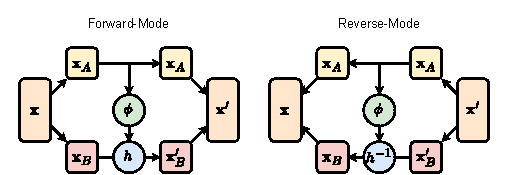
\includegraphics[width=0.8\textwidth]{Figures/transformers/coupling.pdf}
    \caption{A diagram of a coupling flow.}
    \label{fig:coupling_flow}
\end{figure}

Note that the layer only transforms $\x_B$ and leaves $\x_A$ unchanged.
Thus, multiple coupling layers are typically stacked together, interleaved with a fixed random permutation layer or a linear flow to mix the elements of $\x$.
Equivalently one could also alternate the mask used to partition $\x$ between coupling layers.
It is standard invertible to set $h$ to be an elementwise transformation for ensure efficiency as most of the expressivity in the layer comes from $\phi$.
Early original coupling flows used an affine transformation for $h$~\cite{RealNVP}, but this required many layers to fit to complex data distributions.
The expressivity of the model can be greatly enhanced using more complex transformations, yet still elementwise bijections, such as rational quadratic splines~\cite{NeuralSplineFlows}.
This is demonstrated by \Cref{fig:moons}, which shows the output at of a flow with 4 coupling layers with spline transformations, each layer can only transform one dimension of the data.

\begin{figure}[ht]
    \centering
    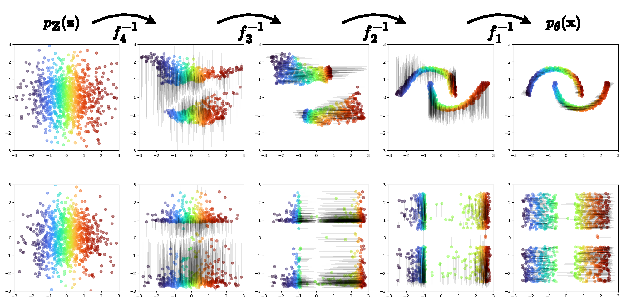
\includegraphics[width=0.95\textwidth]{Figures/transformers/samples.pdf}
    \caption{The transformation of two dimensional Gaussian samples into a double moon distribution using a flow with 4 coupling layers with rational quadratic splines.}
    \label{fig:moons}
\end{figure}

\subsection{Continuous Normalizing Flows}

% In a CNF, the transformation is defined by a differential equation parametrised by a time $t \in [0, 1]$
% Fixed end points are x(0) = 0 and x(1) = z.
% This gives the forward and inverse transformations as two time ordered ODEs,
% Put equation
% Once the transformation is defined, any numerical ODE solver can be used to transform samples from the data space to the latent space and back again.

Whereas in a standard NF the transformation composed by a fixed number of sub-transformations or layers, a continuous normalizing flow (CNF)~\cite{NeuralODE} defines a continuous process where each infinitesimal transformation depends on the current state of the data and the time index.
This leads to an ordinary differential equation (ODE) indexed by a time $t \in [0, 1]$ defined by a smooth time-varying vector field $u(\y, t)$


In a continuous normalizing flow (CNF) the transformation is defined by an ordinary differential equation (ODE) indexed by a time $t \in [0, 1]$.
\begin{equation}
    f(\x) = \x_0 + \int_0^1 u(\x_t, t) \diff t
    \quad \rightarrow \quad
    f^{-1}(\x) = \x_1 + \int_0^1 u(\x_t, t) \diff t.
\end{equation}
Given the distribution of



The fixed end points are $x(0) = 0$ and $x(1) = z$.

Once the transformation is defined, any numerical ODE solver can be used to transform samples from the data space to the latent space and back again.


% CNFs are trained using the same maximum liklihood approach as NFs, but this involves the integral of the trace of the Jaaconian of the transformation
% Put equation
% Quadratic in the dimensions, so not scalable.
% Can use the hutchingson trace estimator.

% The equation prob can also be frames via the continuity equation
% Trace of the jacobian is seen as a divergence of the vector field defined by the transformation
% Can parametrise the vector field with a neural network, and train it to match the data distribution
% Incl equation

% Training via maximum liklihood sucks
% Required an integration over the ODE which not only involves forward pass of the network but a a estimator of divergence too.
% Main issue is how slow they are to train.

\section{Denoising Models}

% Denoising models have taken the world by storm
% They are the current state-of-the-art in generative models
% Initial promise with the iterative refinement paper
% Formailsed in DDPM paper
% Frenzy when they dethroned GANs paper

% Many different, competing, overlapping frameworks to define these models
% Alot of different mathematical derivations for what comes down to the same training objective and practical implementation
% Many attempts to unify these models in a single framework EDM, new CM paper
% We chose to focus on two that were used in projects for this thesis
% Namely score based models and flow matching, focusing on the work by Song, Karras and Lipman.

\subsection{Score-Based Models}

\subsection{Flow Matching}

% CFM and Rectified Flows emerged at the same time
% Flow matching can be seen as an extension of continuous time normalising flows
% Provides a simulatio-free way to train CNF models
% The loss is based on a regression objective to match the correct velocity field
% Include equation
% We reach the same probjem with score-matching, that if we have the field as targets then we dont need to approximate it
% Like with score matching we devise a target without having to calculate the velocity field directly, through denoising.

% Use a latent variable and define the probability path over a joint
% Include equation
% Probability path is a joint over a conditional probability path
% Induces a new continuity equation








\subsection{Consistency Models}
